\documentclass[tikz,border=10pt]{standalone}
\usetikzlibrary{positioning, arrows.meta, decorations.pathreplacing, shapes.geometric}

\begin{document}
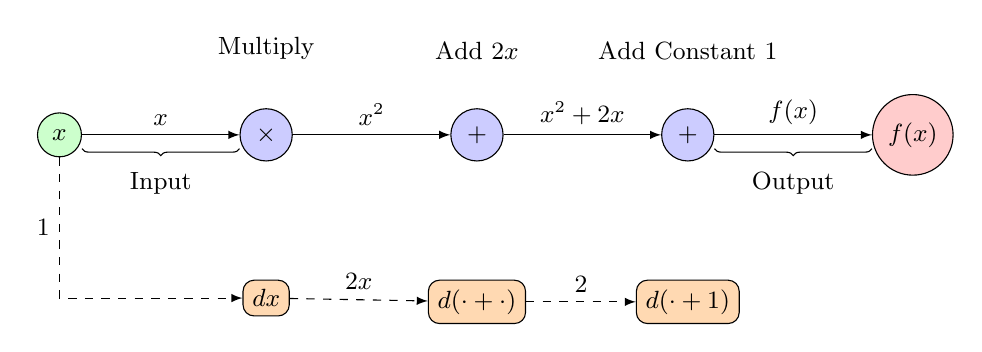
\begin{tikzpicture}[
    node distance=1.5cm and 2cm,
    operation/.style={circle, draw, fill=blue!20},
    input/.style={circle, draw, fill=green!20},
    output/.style={circle, draw, fill=red!20},
    dual/.style={rectangle, draw, rounded corners, fill=orange!30},
    auto/.style={->, >=latex},
    every node/.style={font=\small}
]

% Nodes
\node[input] (x) {$x$};
\node[operation, right=of x] (square) {$\times$};
\node[operation, right=of square] (add) {$+$};
\node[operation, right=of add] (add1) {$+$};
\node[output, right=of add1] (f) {$f(x)$};

\node[dual, below=of square] (dx) {$dx$};
\node[dual, below=of add] (dadd) {$d(\cdot+\cdot)$};
\node[dual, below=of add1] (dadd1) {$d(\cdot+1)$};

% Edges
\draw[auto] (x) -- (square) node[midway, above] {$x$};
\draw[auto] (square) -- (add) node[midway, above] {$x^2$};
\draw[auto] (add) -- (add1) node[midway, above] {$x^2 + 2x$};
\draw[auto] (add1) -- (f) node[midway, above] {$f(x)$};

\draw[auto, dashed] (x) |- (dx) node[near start, left] {1};
\draw[auto, dashed] (dx) -- (dadd) node[midway, above] {2$x$};
\draw[auto, dashed] (dadd) -- (dadd1) node[midway, above] {2};

% Annotations
\node[above=0.5cm of square] (mult) {Multiply};
\node[above=0.5cm of add] (add2x) {Add $2x$};
\node[above=0.5cm of add1] (addConst) {Add Constant $1$};

\draw[decoration={brace, mirror, raise=5pt}, decorate] (x) -- (square) node[midway, below=10pt] {Input};
\draw[decoration={brace, raise=5pt}, decorate] (f) -- (add1) node[midway, below=10pt] {Output};

\end{tikzpicture}
\end{document}
